The next stage of the project was designing a suitable database schema and then performing the migration process.
This milestone was split into multiple parts: choosing the most suitable database solution,
designing the database schema itself, and migration.


\section{Database Solution}\label{sec:database-solution}

The first step in this milestone was choosing the most suitable database solution
that was also most applicable to the use case of this project.
Three candidates were considered: MySQL, PostgreSQL, and MariaDB\@.
Early on,
MySQL was thought
to be obsolete since a lot of its features had been migrated into MariaDB
and was now its subsidiary so that was eliminated immediately.
The two remaining options, PostgreSQL and MariaDB, had their own advantages and disadvantages.
In summary,
PostgreSQL was supported by a vibrant community
but also had known performance issues on large amounts of data
(such as the pull request JSON information)
and problems with compatibility since not all open-source applications support it.
On the other hand,
MariaDB had recently made MySQL a subsidiary which meant it already had an array of great features to offer.
The first complaint made about MariaDB was surrounding the user interface,
which would not be a problem for this project anyway
since queries would mostly be done through the command line or through GUIs within IDEs.
The second was negative performance impacts on large tables with multiple indices.
However, this was not a major concern for development since the pull request data would only
(ideally) need to be migrated once and then never again,
so the performance impacts would not be very noticeable.
Taking into account all the pros and cons, MariaDB was the ultimate choice for the project's database solution due to the overwhelming praise from the community and the plethora of features.


\section{Database Schema}\label{sec:database-schema}

The second step was designing a database schema
to store the pull request information that had been crawled in the previous stage.
Initially, the idea was to have two tables: one for pull requests themselves,
and another for the comments on those pull requests.
However,
this is not a complete solution
since this schema can be further normalised to include individual author information in a separate table.
As a result, a third table is introduced to help make database queries more efficient: the authors table.
Furthermore,
to allow the project to easily expand,
a fourth table was implemented: the projects table.
Each of these four tables contains indices for every non-timestamp column to allow for fast data retrieval.
The final piece of the puzzle was taking advantage of foreign key attributes in every table
to reduce the number of columns required.
Regardless of the issues this may have caused later on,
it was a worthy investment of the milestone since it made backend data retrieval a lot better later on.
A full image of the complete schema in the form of an ER diagram is shown in the Figure~\ref{fig:schema}.

% Will be replaced with figure of ER diagram later on (!!!)
\begin{figure}[h]
    \centering
    \fboxsep 2mm
    \framebox{
        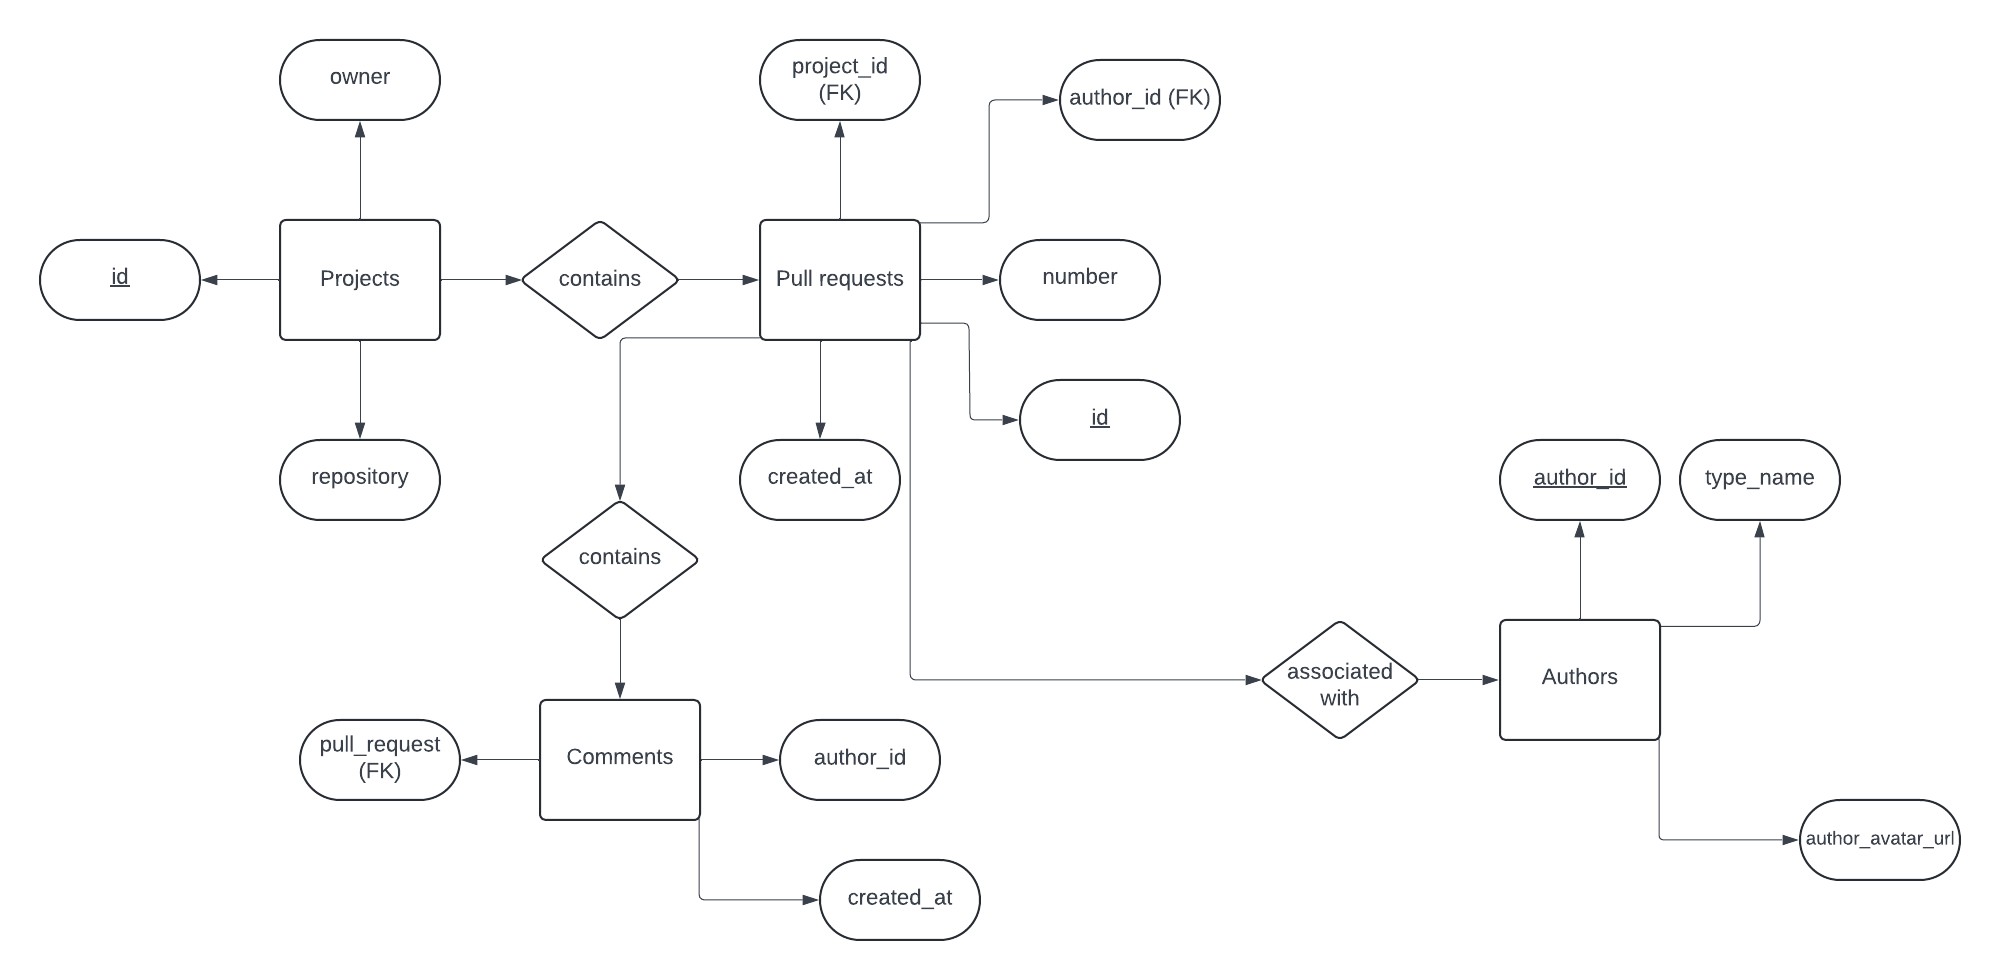
\includegraphics[width=15cm]{schema}
    }
    \caption{\label{fig:schema} ER diagram of final database schema.}
\end{figure}


\section{Migration}\label{sec:migration}

After the schema itself had been formed, the third and final step was storing the data.
This, of course, could not be done manually due to the immense amount of data that was crawled
(17,000+ pull requests, to be exact).
The easiest way to automate this process was with a Python script
that took advantage of the mysql-connector-python pip library.
The biggest roadblock
introduced when manipulating the contents of the schema was navigating the foreign key constraints.
There were many exceptions
that were thrown repeatedly throughout the development of this script because of these constraints.
After much debugging,
the best and most efficient solution was
to partially add column values that did not rely on another table first before adding the rest.
Another problem was deleted GitHub users,
which caused problems since the author object inside the individual crawled JSON files did not exist.
To counteract this issue,
a ``Ghost'' user was added to the authors table during the instantiation of the database schema as a placeholder value for any deleted users.
To avoid adding any duplicate users to the authors table,
there was an internal list
stored within the script
that was compared against every time a pull request author was retrieved from the JSON data.
This process was then repeated for each comment in every pull request to ensure no data redundancy/repetition.
All these changes combined resulted in an efficient migration script
that avoided data redundancy/repetition and foreign key constraint issues along the way.